\section{Review of statistical inference; 2-sample t}
\frame{\sectionpage}





\begin{frame}{The statistical world}
  \begin{itemize}
  \item 
  Consists of:

  \begin{itemize}
  \item objects or people of interest to us ({\em individuals})
  \item things measured or counted on those individuals ({\em variables})
  \end{itemize}

\pause

\item About the individuals:

\begin{itemize}
\item which ones do we care about? All of them, the {\em population}.
\item which ones do we know about? The ones we happened to look at, the {\em sample}.
\end{itemize}

\pause

\item Sample is (or should be) randomly chosen from population, with no favoritism.
  \end{itemize}

\end{frame}

\begin{frame}{Sample to population: confidence interval}
  
  \begin{itemize}
  \item 
Want to know about population (parameter), but don't. Only have sample (statistic). Eg.\ population mean, only have sample mean.
\item Logic:
  \begin{itemize}
  \item {\em If} we knew about population, could figure out kinds of samples that might appear (math).
  \item In particular, can figure how far apart sample statistic and population parameter might be.
  \item Use this to construct {\em confidence interval} for population parameter: says eg.\ ``based on my sample, I think population mean between $a$ and $b$''. 
  \end{itemize}
\end{itemize}
\end{frame}

\begin{frame}[fragile]{Example of confidence interval}
  
  \begin{itemize}
  \item Take a sample of $n=10$ observations. Obtain sample mean of
    $\bar{x}=15$, and sample SD of $s=2.5$. Want 95\% confidence
    interval for population mean.
  \item For population mean \emph{with population SD unknown}: use $t$
    distribution with $n-1=9$ degrees of freedom.
  \item Obtain $t^*$ from $t$-table or as
\begin{knitrout}
\definecolor{shadecolor}{rgb}{0.969, 0.969, 0.969}\color{fgcolor}\begin{kframe}
\begin{alltt}
\hlstd{t.star}\hlkwb{=}\hlkwd{qt}\hlstd{(}\hlnum{1}\hlopt{-}\hlnum{0.05}\hlopt{/}\hlnum{2}\hlstd{,}\hlnum{9}\hlstd{) ; t.star}
\end{alltt}
\begin{verbatim}
[1] 2.262157
\end{verbatim}
\end{kframe}
\end{knitrout}
\item and thus 95\% CI for mean is this: $m=t^* s / \sqrt{n}$, then
  $\bar{x} \pm m$:
\begin{knitrout}
\definecolor{shadecolor}{rgb}{0.969, 0.969, 0.969}\color{fgcolor}\begin{kframe}
\begin{alltt}
\hlstd{m}\hlkwb{=}\hlstd{t.star}\hlopt{*}\hlnum{2.5}\hlopt{/}\hlkwd{sqrt}\hlstd{(}\hlnum{10}\hlstd{) ; m}
\end{alltt}
\begin{verbatim}
[1] 1.788392
\end{verbatim}
\begin{alltt}
\hlkwd{c}\hlstd{(}\hlnum{15}\hlopt{-}\hlstd{m,}\hlnum{15}\hlopt{+}\hlstd{m)}
\end{alltt}
\begin{verbatim}
[1] 13.21161 16.78839
\end{verbatim}
\end{kframe}
\end{knitrout}
  \end{itemize}
  
\end{frame}

\begin{frame}{Test of significance}
\begin{itemize}
\item Or: 
  \begin{itemize}
  \item 
might have theory leading to {\em null hypothesis} (eg.\ population mean is 20) and {\em alternative hypothesis} (eg.\ population mean not 20).
\item This leads to {\em test of significance} (hypothesis test): ``based on my sample, I think pop.\ mean is (is not) 20''
\item Done by choosing $\alpha$ (eg.\ 0.05), calculating {\em test statistic} and {\em P-value}. If P-value $< \alpha$, {\em reject null}: have evidence in favour of alternative.
  \end{itemize}
\item Math producing inference procedures can be difficult, but calculations (with software) and interpretations need not be.
  \end{itemize}


\end{frame}

\begin{frame}[fragile]{Example of test of significance}
  
  
  \begin{itemize}
  \item   Let's suppose we are trying to prove that a population mean is not
  equal to 17 (alternative hypothesis), against a null that the mean
  is 17 after all. Use $\alpha=0.05$.
\item Use same data as before: $n=10, \bar{x}=15, s=2.5$.
\item Calculate test statistic $t=(\bar{x}-\mu_0)/(s/\sqrt{n})$, where
  $\mu_0$ is the population mean given by the null hypothesis:
\begin{knitrout}
\definecolor{shadecolor}{rgb}{0.969, 0.969, 0.969}\color{fgcolor}\begin{kframe}
\begin{alltt}
\hlstd{t.stat}\hlkwb{=}\hlstd{(}\hlnum{15}\hlopt{-}\hlnum{17}\hlstd{)}\hlopt{/}\hlstd{(}\hlnum{2.5}\hlopt{/}\hlkwd{sqrt}\hlstd{(}\hlnum{10}\hlstd{)) ; t.stat}
\end{alltt}
\begin{verbatim}
[1] -2.529822
\end{verbatim}
\end{kframe}
\end{knitrout}
\item Get P-value by looking along 9 df row of $t$-table, and seeing
  where \texttt{t.tstat}, or its absolute value, comes. Or get P-value
  directly from R. \emph{left} tail here, since
  \texttt{t.stat} $<0$; also $\times 2$ for
  two-sided test:
\begin{knitrout}
\definecolor{shadecolor}{rgb}{0.969, 0.969, 0.969}\color{fgcolor}\begin{kframe}
\begin{alltt}
\hlnum{2}\hlopt{*}\hlkwd{pt}\hlstd{(t.stat,}\hlnum{9}\hlstd{)}
\end{alltt}
\begin{verbatim}
[1] 0.03224478
\end{verbatim}
\end{kframe}
\end{knitrout}
  \end{itemize}
  
\end{frame}

\begin{frame}[fragile]{Conclusion}
  
  \begin{itemize}
  \item $\alpha=0.05$, P-value was 0.032.
  \item P-value less than $\alpha$, so \emph{reject} null hypothesis
    in favour of alternative: that is, population mean \emph{not} equal to 17.
  \item If had $\alpha=0.01$, would not have been able to reject
    null. So evidence against a mean of 17 is strong but not
    \emph{that} strong.
  \end{itemize}
\end{frame}

\begin{frame}[fragile]{Doing it in R}
  


\begin{itemize}
\item These data have right mean and SD:
\begin{knitrout}
\definecolor{shadecolor}{rgb}{0.969, 0.969, 0.969}\color{fgcolor}\begin{kframe}
\begin{alltt}
\hlstd{mydata}
\end{alltt}
\begin{verbatim}
 [1] 18.99229 15.25282 11.22454 14.66774
 [5] 14.89869 14.34578 16.47864 10.89571
 [9] 17.38091 15.86289
\end{verbatim}
\end{kframe}
\end{knitrout}
\item One step with R (note everything as before):
  {\small
\begin{knitrout}
\definecolor{shadecolor}{rgb}{0.969, 0.969, 0.969}\color{fgcolor}\begin{kframe}
\begin{alltt}
\hlkwd{t.test}\hlstd{(mydata,}\hlkwc{mu}\hlstd{=}\hlnum{17}\hlstd{)}
\end{alltt}
\begin{verbatim}

	One Sample t-test

data:  mydata
t = -2.5298, df = 9, p-value = 0.03224
alternative hypothesis: true mean is not equal to 17
95 percent confidence interval:
 13.21161 16.78839
sample estimates:
mean of x 
       15 
\end{verbatim}
\end{kframe}
\end{knitrout}
}
\end{itemize}
  
\end{frame}

\begin{frame}{Exploratory data analysis}
  \begin{itemize}
  \item Sometimes don't have theory (yet), just want to see what data
    tell us.
  \item Use graphs, simple descriptive statistics, some of methods we learn.
  \item Idea: generate ideas (``hypotheses'') for future study.
  \item Cannot make clear conclusions about populations.
  \end{itemize}
\end{frame}


\begin{frame}{The Degree of Reading Power data}

  \begin{itemize}
  \item Have new method for teaching reading.
  \item Want to see if better than ``standard'' method (``research hypothesis'').
  \item Design: randomly allocate available children to ``treatment''
    (new method) or ``control'' (standard).
  \item Measure score for all children on standard reading test.
  \item Analysis: is observed difference between treatment/control score
    means big enough to be real not chance? Do 2-sample $t$-test.
  \end{itemize}

\end{frame}

\begin{frame}[fragile]{Some of the data}

\begin{verbatim}
t 43
t 53
t 57
t 49
t 56
t 33
c 42
c 33
c 46
c 37
c 43
\end{verbatim}

  \begin{itemize}
  \item 1st column label (``t'' for treatment, ``c'' for control).
  \item 2nd column response (score on reading test).
  \item Data in plain text file \verb-drp.txt-.

  \end{itemize}
  
\end{frame}


\begin{frame}[fragile]{Reading and examining data}
  
 
\begin{knitrout}
\definecolor{shadecolor}{rgb}{0.969, 0.969, 0.969}\color{fgcolor}\begin{kframe}
\begin{alltt}
\hlstd{drp}\hlkwb{=}\hlkwd{read.table}\hlstd{(}\hlstr{"drp.txt"}\hlstd{,}\hlkwc{header}\hlstd{=T)}
\hlkwd{head}\hlstd{(drp)}
\end{alltt}
\begin{verbatim}
  group score
1     t    24
2     t    61
3     t    59
4     t    46
5     t    43
6     t    44
\end{verbatim}
\end{kframe}
\end{knitrout}

\begin{itemize}
\item \texttt{read.table} gets data from ``space-delimited'' text
  file. \texttt{header=T} reads top line as variable names.
\item Resulting R data structure called \texttt{data.frame}, basic
  arrangement for data in R.
\item \texttt{head} looks at first few lines (default 6) of data frame.
\end{itemize}

 
\end{frame}

\begin{frame}[fragile]{Visual comparison of groups}
  
  \begin{itemize}
  \item My favourite tool: \textbf{boxplot}:
    
\begin{knitrout}
\definecolor{shadecolor}{rgb}{0.969, 0.969, 0.969}\color{fgcolor}\begin{kframe}
\begin{alltt}
\hlstd{gbox}\hlkwb{=}\hlkwd{ggplot}\hlstd{(drp,}\hlkwd{aes}\hlstd{(}\hlkwc{x}\hlstd{=group,}\hlkwc{y}\hlstd{=score))}\hlopt{+}\hlkwd{geom_boxplot}\hlstd{()}
\hlstd{gbox}
\end{alltt}
\end{kframe}
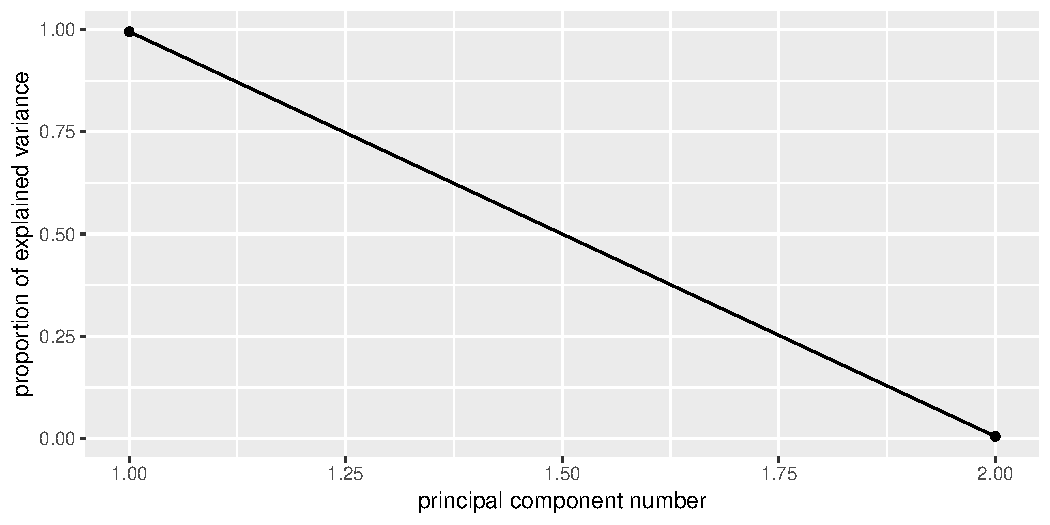
\includegraphics[width=\maxwidth]{figure/unnamed-chunk-8-1} 

\end{knitrout}
    

  \end{itemize}
  
\end{frame}



\begin{frame}[fragile]{Comments and setup}
  
  \begin{itemize}
  \item Mean reading score for treatment group is higher
  \item but a lot of variability.
  \item Is that difference real/reproducible?
  \item Do \emph{two-sample $t$-test}.
  \item \textbf{P-value} tells you whether difference in samples
    likely to persist in population
  \item Small P-value (less than 0.05) means ``yes, it's real''
  \item Confidence interval says how far apart means might be.
  \end{itemize}
  
\end{frame}

\begin{frame}[fragile]{Two-sample $t$}

{\small

 
\begin{knitrout}
\definecolor{shadecolor}{rgb}{0.969, 0.969, 0.969}\color{fgcolor}\begin{kframe}
\begin{alltt}
\hlkwd{with}\hlstd{(drp,}\hlkwd{t.test}\hlstd{(score}\hlopt{~}\hlstd{group))}
\end{alltt}
\begin{verbatim}

	Welch Two Sample t-test

data:  score by group
t = -2.3109, df = 37.855, p-value =
0.02638
alternative hypothesis: true difference in means is not equal to 0
95 percent confidence interval:
 -18.67588  -1.23302
sample estimates:
mean in group c mean in group t 
       41.52174        51.47619 
\end{verbatim}
\end{kframe}
\end{knitrout}

}

\begin{itemize}
\item P-value 0.026 says means really are different
\item CI says difference between 1 and 19 points in favour of new
  reading program.
\item R puts groups in alphabetical order (\texttt{c} before \texttt{t}).
\end{itemize}

\end{frame}


\begin{frame}{Comments}

  \begin{itemize}
  \item New reading program really helps!
  \item 2 possible $t$ procedures:
    \begin{itemize}
    \item Pooled: assumes 2 population variances/SDs are same
    \item Welch/Satterthwaite: does not, but only approximation.
    \end{itemize}
  \item R does Welch by default. If willing to assume equal variances,
    add \texttt{var.equal=T} to \texttt{t.test}.
  \end{itemize}
  
\end{frame}
